\documentclass[12pt,twoside]{report}

% for the TODOS
\usepackage{todonotes}\usepackage{todonotes}

\usepackage[utf8]{inputenc}
\usepackage[style=numeric]{biblatex}
\bibliography{references}
\renewcommand*{\bibfont}{\normalfont\footnotesize}  % reduce the font size of the bibliography
\usepackage{hyperref}
\usepackage{graphicx}
\usepackage{array}
\usepackage{paralist}
\usepackage{listings}
\usepackage{amsmath}
\usepackage{amssymb}
\usepackage{chngcntr}
\counterwithout{equation}{chapter} % remove the chapter number
\usepackage{subcaption}
\usepackage{fancyhdr}
\usepackage{geometry}

% footnote always at the bottom of the page
\usepackage[bottom]{footmisc}

\usepackage{tabularx}
\newcolumntype{Y}{>{\centering\arraybackslash}X}

\usepackage[chapter]{algorithm}
\usepackage{algpseudocode}
\algrenewcommand{\alglinenumber}[1]{\color{gray}\footnotesize#1:}

\newcommand {\mvd}{\mbox{$\; \rightarrow \! \! \! \! \rightarrow \; $}}    % multi-valued dependency
\DeclareMathOperator*{\argmax}{argmax}    % add argmax to math mode
\DeclareMathOperator*{\argmin}{argmin}    % add argmin to math mode

% names for autoref
\newcommand{\algorithmautorefname}{Algorithm}
\newcommand{\exampleautorefname}{Example}
\renewcommand{\sectionautorefname}{Section}
\renewcommand{\subsectionautorefname}{Subsection}

% environment: definition
\newcounter{definition}
\newenvironment{definition}[1][]{\refstepcounter{definition}\par\medskip
   \noindent \textbf{Definition~\thedefinition~(#1).} \rmfamily\itshape}{\par\medskip}

% environment: heuristic
\newcounter{heuristic}
\newenvironment{heuristic}[1][]{\refstepcounter{heuristic}\par\medskip
   \noindent \textbf{Heuristic~\theheuristic~(#1).} \rmfamily\itshape}{\par\medskip}

% environment: example   
\newcounter{example}[section]
\newenvironment{exmp}[1][]{\refstepcounter{example}\par\bigskip
   \noindent \textbf{Example~\theexample} \rmfamily\itshape}{\par\bigskip}

% image base path
\graphicspath{{images/}}

% listing style for SPARQL queries
\lstdefinestyle{sparql}{
    basicstyle=\scriptsize,
    frame=tb,
    keywordstyle=\bfseries,
    morekeywords={PREFIX, SELECT, DISTINCT, UNION, OPTIONAL, FILTER, WHERE}
}

\lstdefinestyle{base}{
    basicstyle=\footnotesize,
    morecomment=[f][\color{olive}][0]{\#},
}

% color definitions
\definecolor{lightblue}{RGB}{33,204,219}
\definecolor{darkgreen}{RGB}{0,166,0}

% for the inspirational quote
\usepackage{epigraph}
\setlength\epigraphwidth{\textwidth}
\setlength\epigraphrule{0pt}

% for the date
%\usepackage{datetime}
%\newdateformat{monthyeardate}{\monthname[\THEMONTH], \THEYEAR}

% blankpage
\usepackage{afterpage}
\newcommand\blankpage{%
    \null
    \thispagestyle{empty}%
    \addtocounter{page}{-1}%
    \newpage}

\newcommand{\addtotoc}[1]{\addcontentsline{toc}{chapter}{#1}}

% image positioning on cover
\usepackage[absolute]{textpos}

% acronyms
\usepackage[nopostdot,nonumberlist,acronym]{glossaries}
\makenoidxglossaries
\newacronym{rdf}{RDF}{Resource Description Framework}
\newacronym{uri}{URI}{Universal Resource Identifier}
%\newacronym{iri}{IRI}{Internationalized Resource Identifier}
\newacronym{rdfs}{RDFS}{RDF Schema}
%\newacronym{w3c}{W3C}{World Wide Web Consortium}
%\newacronym{rml}{RML}{RDF Mapping Language}
\newacronym{rdfmt}{RDF-MT}{RDF Molecule Template}
\newacronym{gav}{GaV}{Global-as-View}
\newacronym{glav}{GLaV}{Global-Local-as-View}
\newacronym{lav}{LaV}{Local-as-View}
\newacronym{sdl}{SDL}{Semantic Data Lake}
\newacronym{qep}{QEP}{Query Execution Plan}
%\newacronym{dp}{DP}{Dynamic Programming}
\newacronym{lslod}{LSLOD}{Life Science Linked Open Data}
\newacronym{ssq}{SSQ}{star-shaped sub-query}

\renewcommand*{\lstlistlistingname}{List of Listings}  % change the header of the list of listings

\usepackage{adjustbox}
\usepackage{rotating}

\begin{document}
\pagenumbering{Roman}


\newgeometry{left=1.15in, right=1.15in}
\begin{titlepage}
    \centering
    \begin{textblock*}{165mm}(25mm,12.5mm)
        
\includegraphics[height=1.75cm]{logos/logo_luh.jpg} \hfill 
\includegraphics[height=1.75cm]{logos/logo_tib.png}
    \end{textblock*}
    
    \vspace*{1.5em}
    
    {\scshape\Large \href{www.uni-hannover.de}{Gottfried Wilhelm Leibniz Universität Hannover}\par}
    {\scshape\large \href{www.et-inf.uni-hannover.de}{Fakultät für Elektrotechnik und Informatik}\par}
    
    \vfill
    
    {\LARGE\bfseries Information extraction from arcticles on the impacts of COVID-19 lockdowns on air quality \par}
    
    \vfill
    
    {\textit{A thesis submitted in fulfillment of the requirements for the degree of}\par}
    {\textbf{Bachelor of Science in Computer Science}\par}
    
    \vspace*{2em}
    {BY\par}
    \vspace*{2em}
    
    {\bfseries\large Quentin Münch\par}
    {Matriculation number: 10031323\par}
    {E-mail: quentin.muench@stud.uni-hannover.de\par}
    
    \vspace*{2.5em}
    
    {First evaluator: Prof. Dr. Sören Auer\par}
    {Second evaluator: Dr. Jennifer D'Souza\par}
    {Supervisor: Dr. Markus Stocker}
    
    \vfill
    
    %{\Large \monthyeardate\today\par}
    %{\Large \today\par}
    {\Large 31.08.2022}
    
    \vspace*{2.5cm}
    
    \begin{textblock*}{165mm}(25mm,220mm)
        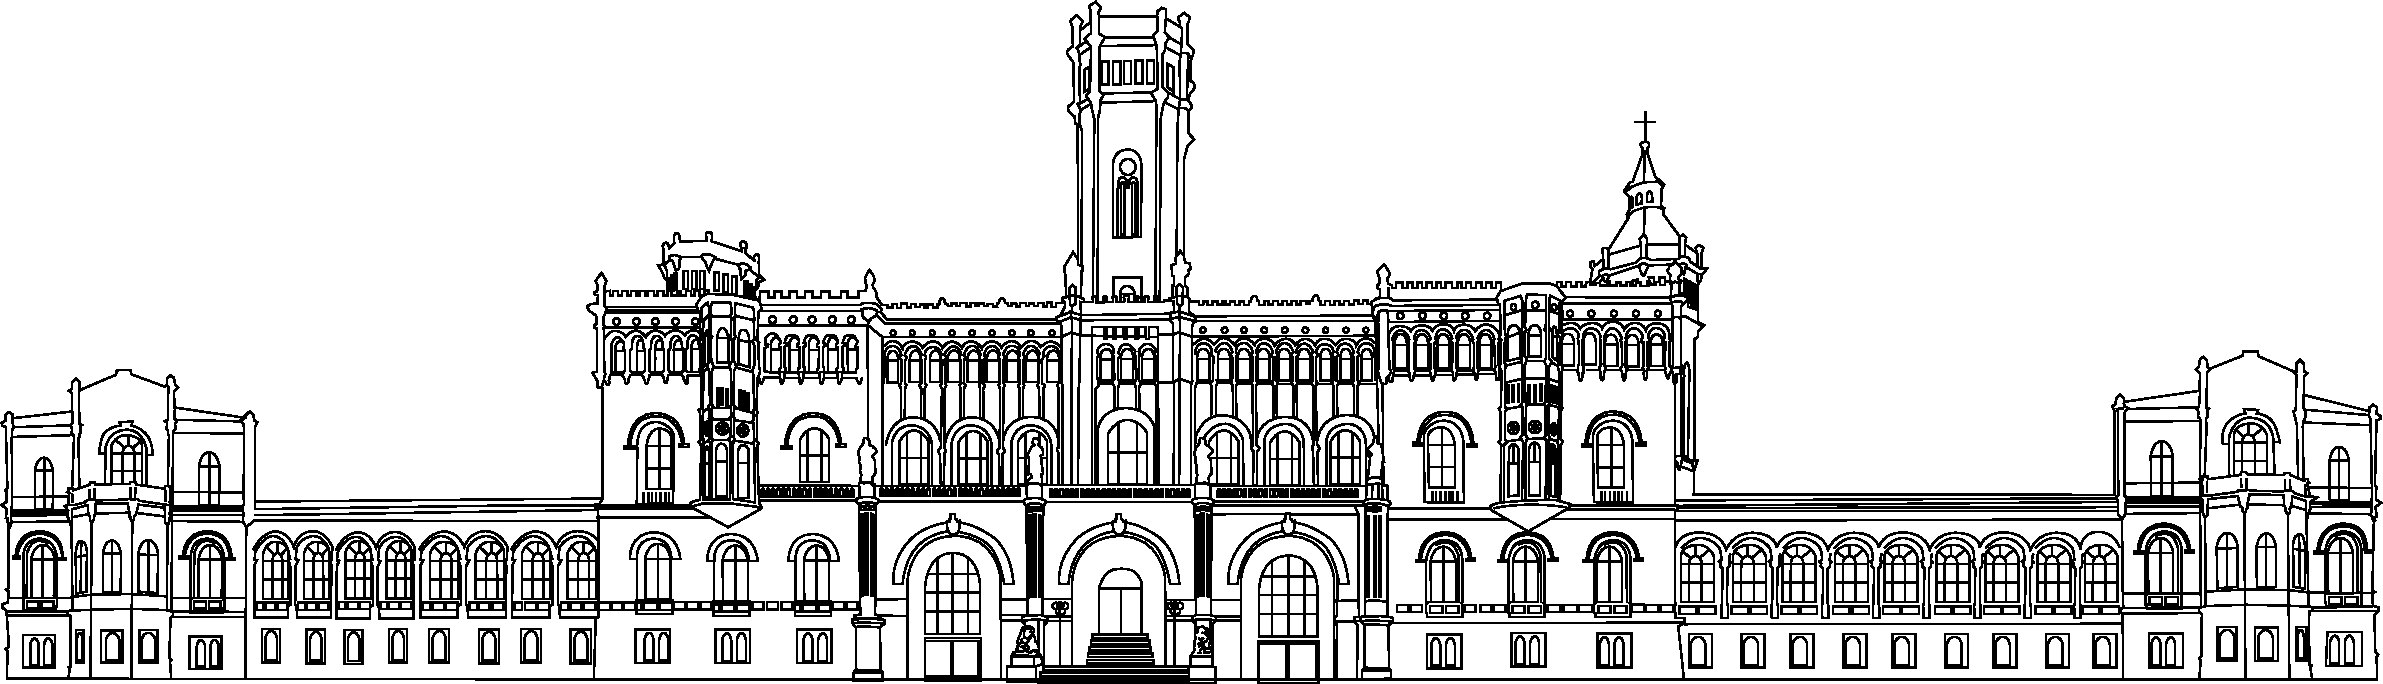
\includegraphics[width=165mm]{logos/welfenschloss.pdf}
    \end{textblock*}
\end{titlepage}

\clearpage
\restoregeometry           %% title page
\blankpage

\newpage
\setcounter{page}{1}
\begin{center}
    \Large
    \textbf{Declaration of Authorship}
\end{center}

\vspace*{1em}

\noindent I, Quentin Münch, declare that this thesis titled, 'Information extraction from articles on the impact of COVID-19 lockdowns on air quality' and the work presented in it are my own. I confirm that:

\vspace*{3em}

\begin{itemize}
    \item This work was done wholly or mainly while in candidature for a research degree at this University.
    \item Where any part of this thesis has previously been submitted for a degree or any other qualification at this University or any other institution, this has been clearly stated.
    \item Where I have consulted the published work of others, this is always clearly attributed.
    \item Where I have quoted from the work of others, the source is always given. With the exception of such quotations, this thesis is entirely my own work.
    \item I have acknowledged all main sources of help.
\end{itemize}

\vspace*{2.5em}

\noindent NAME \\ \\
\begin{tabular}{@{}p{.72in}p{3.0in}@{}}
    Signature: & \hrulefill \\
    &\\
    Date:   & \hrulefill
\end{tabular}
          %% declaration of authorship
\afterpage{\blankpage}

\newpage
\thispagestyle{empty}
%\todo[inline]{decide for one quote}
%\epigraph{``quote"}{--- \textup{author}, where/work}
%\epigraph{``If you believe it will work out, you'll see opportunities. If you believe it won't, you will see obstacles."}{--- \textup{Wayne Dyer}}
%\epigraph{``Start by doing what's necessary; then do what's possible; and suddenly you are doing the impossible."}{--- \textup{Francis of Assisi}}
%\epigraph{``Nothing shocks me. I'm a scientist."}{--- \textup{Indiana Jones}, movie \textit{Indiana Jones and the Temple of Doom} (1984)}
%\epigraph{``Swordfighting is a little like making love. It's not always what you do, but what you say."}{--- \textup{Sword Teacher}, video game \textit{The Secret of Monkey Island} (1990)}
~
\vfill
OPTIONAL


\vfill
~
 %% inspirational quote
\afterpage{\blankpage}

\newpage
\begin{center}
    \Large
    \textit{Acknowledgements}
\end{center}

\vspace*{1cm}

XXXXX
     %% acknowledgments
\afterpage{\blankpage}

\newpage
\begin{center}
    \Large
    \textit{Abstract}
\end{center}

\vspace*{1cm}

\noindent Your Abstract. Clearly motivate your work (WHY), state what is your problem (WHAT), and describe your solution (HOW). Also, explain how your solution was evaluated (either empirically or formally) and summarized the observed results 
~

\noindent\textit{Keywords: KW1, KW2, KWn}

\afterpage{\blankpage}

\tableofcontents
{\small\listoffigures}
{\small\listoftables}
%{\small\lstlistoflistings}
%{\small\listofalgorithms}

\glsaddall
{\small\printnoidxglossaries}

\afterpage{\blankpage}
\newpage

%% set the page style
\pagestyle{fancy}
\fancyhead[R,C,L]{}
%\fancyhead[RE]{\small{ \emph{\nouppercase{\leftmark}}}}
%\fancyhead[LO]{\small \emph{\nouppercase{\rightmark}}}
\fancyhead[RE]{\small{\nouppercase{\leftmark}}}
\fancyhead[LO]{\small{\nouppercase{\rightmark}}}
\fancyfoot[L,R]{}
\fancyfoot[C]{\thepage}
\renewcommand{\headrulewidth}{1pt}
\renewcommand{\footrulewidth}{0pt}
\setlength{\headheight}{14pt}

\pagenumbering{arabic}
\chapter{Introduction}
Your Introduction
%%%%%%%%%%%%%%%%%%%%%%%%%%%%%%%%%%%%%%%%%%%%%%%%%%%%%%%%%%%%%%%%%%%%%%%%%%%%%%%%%%%%%%%%%%%%%%
%%                                                                                          %%
%%                                    WHY                                   %%
%%                                                                                          %%
%%%%%%%%%%%%%%%%%%%%%%%%%%%%%%%%%%%%%%%%%%%%%%%%%%%%%%%%%%%%%%%%%%%%%%%%%%%%%%%%%%%%%%%%%%%%%%


%%%%%%%%%%%%%%%%%%%%%%%%%%%%%%%%%%%%%%%%%%%%%%%%%%%%%%%%%%%%%%%%%%%%%%%%%%%%%%%%%%%%%%%%%%%%%%
%%                                                                                          %%
%%                                    Motivating Example                                    %%
%%                                                                                          %%
%%%%%%%%%%%%%%%%%%%%%%%%%%%%%%%%%%%%%%%%%%%%%%%%%%%%%%%%%%%%%%%%%%%%%%%%%%%%%%%%%%%%%%%%%%%%%%



%%%%%%%%%%%%%%%%%%%%%%%%%%%%%%%%%%%%%%%%%%%%%%%%%%%%%%%%%%%%%%%%%%%%%%%%%%%%%%%%%%%%%%%%%%%%%%
%%                                                                                          %%
%%                                      Contributions                                       %%
%%                                                                                          %%
%%%%%%%%%%%%%%%%%%%%%%%%%%%%%%%%%%%%%%%%%%%%%%%%%%%%%%%%%%%%%%%%%%%%%%%%%%%%%%%%%%%%%%%%%%%%%%
%%%%%%%%%%%%%%%%%%%%%%%%%%%%%%%%%%%%%%%%%%%%%%%%%%%%%%%%%%%%%%%%%%%%%%%%%%%%%%%%%%%%%%%%%%%%%%
%%                                                                                          %%
%%                                    Structure of the Book                                      %%
%%                                                                                          %%
%%%%%%%%%%%%%%%%%%%%%%%%%%%%%%%%%%%%%%%%%%%%%%%%%%%%%%%%%%%%%%%%%%%%%%%%%%%%%%%%%%%%%%%%%%%%%%



\chapter{Background}
This chapter introduces the main topics needed to understand the development of this thesis.

%%%%%%%%%%%%%%%%%%%%%%%%%%%%%%%%%%%%%%%%%%%%%%%%%%%%%%%%%%%%%%%%%%%%%%%%%%%%%%%%%%%%%%%%%%%%%%
%%                                                                                          %%
%%                                Semantic Web Technologies                                 %%
%%                                                                                          %%
%%%%%%%%%%%%%%%%%%%%%%%%%%%%%%%%%%%%%%%%%%%%%%%%%%%%%%%%%%%%%%%%%%%%%%%%%%%%%%%%%%%%%%%%%%%%%%


\chapter{Related Work}
%There has been a lot of research in topics related to this thesis.
Topics related to this thesis have been extensively treated in the literature.
This chapter presents an overview of what has been done 


\chapter{Approach}
This chapter states the problem statement and proposed solution


%%%%%%%%%%%%%%%%%%%%%%%%%%%%%%%%%%%%%%%%%%%%%%%%%%%%%%%%%%%%%%%%%%%%%%%%%%%%%%%%%%%%%%%%%%%%%%
%%                                                                                          %%
%%                                    Problem Statement                                     %%
%%                                                                                          %%
%%%%%%%%%%%%%%%%%%%%%%%%%%%%%%%%%%%%%%%%%%%%%%%%%%%%%%%%%%%%%%%%%%%%%%%%%%%%%%%%%%%%%%%%%%%%%%
%%%%%%%%%%%%%%%%%%%%%%%%%%%%%%%%%%%%%%%%%%%%%%%%%%%%%%%%%%%%%%%%%%%%%%%%%%%%%%%%%%%%%%%%%%%%%%
%%                                                                                          %%
%%                                    Proposed Solution                                     %%
%%                                                                                          %%
%%%%%%%%%%%%%%%%%%%%%%%%%%%%%%%%%%%%%%%%%%%%%%%%%%%%%%%%%%%%%%%%%%%%%%%%%%%%%%%%%%%%%%%%%%%%%%

\chapter{Implementation}
This section presents your implementation


\chapter{Experimental Evaluation}\label{sec:experiment}
The experimental evaluation is reported in this section. Please, include your research questions. 

The research questions addressed by this thesis are:
\begin{inparaenum}[\bfseries RQ1)]
    \item YYY
    \item XXX
    \item TT
    \item OPP

\end{inparaenum}
The remainder of this chapter is structured as follows:
First, the used benchmark is described.
Second, the data preparation is presented.
Afterwards, the setup of the experiment is depicted.
Finally, the results are shown and analyzed.


%%%%%%%%%%%%%%%%%%%%%%%%%%%%%%%%%%%%%%%%%%%%%%%%%%%%%%%%%%%%%%%%%%%%%%%%%%%%%%%%%%%%%%%%%%%%%%
%%                                                                                          %%
%%                                       Benchmark                                          %%
%%                                                                                          %%
%%%%%%%%%%%%%%%%%%%%%%%%%%%%%%%%%%%%%%%%%%%%%%%%%%%%%%%%%%%%%%%%%%%%%%%%%%%%%%%%%%%%%%%%%%%%%%

%%%%%%%%%%%%%%%%%%%%%%%%%%%%%%
%    Benchmarking Queries    %
%%%%%%%%%%%%%%%%%%%%%%%%%%%%%%

%%%%%%%%%%%%%%%%%%%%%%%%%%%%%%%%%%%%%%%%%%%%%%%%%%%%%%%%%%%%%%%%%%%%%%%%%%%%%%%%%%%%%%%%%%%%%%
%%                                                                                          %%
%%                                    Data Preparation                                      %%
%%                                                                                          %%
%%%%%%%%%%%%%%%%%%%%%%%%%%%%%%%%%%%%%%%%%%%%%%%%%%%%%%%%%%%%%%%%%%%%%%%%%%%%%%%%%%%%%%%%%%%%%%

%%%%%%%%%%%%%%%%%%%%%%%%%%%%%%%%%%%%%%%%%%%%%%%%%%%%%%%%%%%%%%%%%%%%%%%%%%%%%%%%%%%%%%%%%%%%%%
%%                                                                                          %%
%%                                   Experimental Setup                                     %%
%%                                                                                          %%
%%%%%%%%%%%%%%%%%%%%%%%%%%%%%%%%%%%%%%%%%%%%%%%%%%%%%%%%%%%%%%%%%%%%%%%%%%%%%%%%%%%%%%%%%%%%%%


\textbf{Benchmark:}


\textbf{Metrics:}


\textbf{Implementations:}



%%%%%%%%%%%%%%%%%%%%%%%%%%%%%%%%%%%%%%%%%%%%%%%%%%%%%%%%%%%%%%%%%%%%%%%%%%%%%%%%%%%%%%%%%%%%%%
%%                                                                                          %%
%%                                       Evaluation                                         %%
%%                                                                                          %%
%%%%%%%%%%%%%%%%%%%%%%%%%%%%%%%%%%%%%%%%%%%%%%%%%%%%%%%%%%%%%%%%%%%%%%%%%%%%%%%%%%%%%%%%%%%%%%


\chapter{Conclusions and Future Work}
This  chapter presents the lessons learned and future work


%%%%%%%%%%%%%%%%%%%%%%%%%%%%%%%%%%%%%%%%%%%%%%%%%%%%%%%%%%%%%%%%%%%%%%%%%%%%%%%%%%%%%%%%%%%%%%
%%                                                                                          %%
%%                                       Conculsions                                        %%
%%                                                                                          %%
%%%%%%%%%%%%%%%%%%%%%%%%%%%%%%%%%%%%%%%%%%%%%%%%%%%%%%%%%%%%%%%%%%%%%%%%%%%%%%%%%%%%%%%%%%%%%%


%%%%%%%%%%%%%%%%%%%%%%%%%%%%%%%%%%%%%%%%%%%%%%%%%%%%%%%%%%%%%%%%%%%%%%%%%%%%%%%%%%%%%%%%%%%%%%
%%                                                                                          %%
%%                                      Limitations                                         %%
%%                                                                                          %%
%%%%%%%%%%%%%%%%%%%%%%%%%%%%%%%%%%%%%%%%%%%%%%%%%%%%%%%%%%%%%%%%%%%%%%%%%%%%%%%%%%%%%%%%%%%%%%


%%%%%%%%%%%%%%%%%%%%%%%%%%%%%%%%%%%%%%%%%%%%%%%%%%%%%%%%%%%%%%%%%%%%%%%%%%%%%%%%%%%%%%%%%%%%%%
%%                                                                                          %%
%%                                      Future Work                                         %%
%%                                                                                          %%
%%%%%%%%%%%%%%%%%%%%%%%%%%%%%%%%%%%%%%%%%%%%%%%%%%%%%%%%%%%%%%%%%%%%%%%%%%%%%%%%%%%%%%%%%%%%%%


%%%%%%%%%%%%%%%%%%%%%%%%%%%%%%%%%%%%%%%
%%              APPENDIX             %%
%%%%%%%%%%%%%%%%%%%%%%%%%%%%%%%%%%%%%%%


%%%%%%%%%%%%%%%%%%%%%%%%%%%%%%%%%%%%%%%
%%             REFERENCES            %%
%%%%%%%%%%%%%%%%%%%%%%%%%%%%%%%%%%%%%%%
\pagebreak
\addtotoc{Bibliography}
\printbibliography

\end{document}
